\documentclass[conference]{IEEEtran}
\usepackage{amsmath,amssymb,amsthm}
\usepackage{graphicx}
\usepackage{booktabs}
\usepackage{url}
\usepackage{cite}

\newtheorem{lemma}{Lemma}
\newtheorem{theorem}{Theorem}

% All numbers quoted from experiments come from generated/numbers.tex (see experiments/make_tables_tex.py).
\newcommand{\EOneRows}{168}
\newcommand{\EThreeSlopeGP}{0.44}
\newcommand{\EThreeSlopeRebuild}{1.00}
\newcommand{\EFourMaxHalf}{2.928}
\newcommand{\EFourMaxOne}{2.000}
\newcommand{\EFourMaxTwo}{1.749}


\begin{document}

\title{Certificate-Driven, Budgeted Reoptimization of Shortest-Path Trees\\
with Exact Tour Re-solving for Dynamic Delivery Routing}

\author{\IEEEauthorblockN{GraphPulse-R project team}
\IEEEauthorblockA{Design and Analysis of Algorithms, VIT\\
Draft for team review --- author list and affiliations to be completed}}

\maketitle

\begin{abstract}
When roads close or slow down, a delivery planner must keep shortest-path distances and a delivery tour correct.
We study directed graphs with positive integer weights under a stream of edge deletions and weight increases,
and maintain after every update (i) exact single-source distances from a depot and $k$ stops, (ii) the terminal distance matrix, and (iii) a minimum-cost single-vehicle tour.
We combine three mechanisms: an $O(1)$ structural \emph{certificate} that proves an update leaves a shortest-path tree unchanged;
\emph{budgeted incremental repair}, in which repair of the affected region runs under a work cap $B=\lceil cF\rceil$ ($F$ is the cost of a full rebuild) and is aborted for free on a copy-on-write overlay before a rebuild fallback;
and a \emph{lazy tour certificate} that skips the exact Held--Karp solve when no matrix entry used by the incumbent tour has changed.
We prove a per-update work bound $(1+c)F+2$ and a competitive ratio $\max(1+c,(1+c)/c)$ against the per-update offline optimum, minimised at $c=1$, both for an oracle estimate of $F$.
All variants are cross-checked against a recompute-everything reference after every update, and all results are reported in machine-independent operation counts.
The system integrates known ingredients; we make no claim of a new algorithm.
\end{abstract}

\begin{IEEEkeywords}
dynamic shortest paths, certificates, competitive analysis, reoptimization, vehicle routing
\end{IEEEkeywords}

\section{Introduction}
Last-mile logistics runs on road networks whose costs change. Recomputing every shortest path and the delivery tour after each change is correct but wasteful, because most changes do not affect the current plan.
Two decisions are usually left informal: whether to \emph{repair} or \emph{rebuild} the shortest-path structures after a change, and whether to \emph{re-solve} the tour or keep it.
We make both decisions with checkable certificates and a provable work budget.

\textbf{Contributions.} (1) A decision cascade for maintaining exact shortest-path trees under monotone updates, with an $O(1)$ certificate and alternative-support test.
(2) Abort-free budgeted repair with a rebuild fallback, a work bound, and a ski-rental style competitive analysis, including a randomised budget.
(3) A lazy tour certificate with an $\varepsilon$-tolerant mode whose lower bound is deliberately never raised.
(4) An end-to-end evaluation in operation counts, including adversarial instances that exhibit the tightness of the bound and results where the method gains little.

\section{Related Work}
Dynamic shortest-path maintenance has a long literature, including bounded incremental algorithms~\cite{ramalingam1996} and decremental trees~\cite{evenshiloach1981}.
The Held--Karp dynamic program~\cite{heldkarp1962} solves the travelling-salesman problem exactly, and the underlying Hamiltonian-cycle problem is NP-complete~\cite{karp1972}.
Rent-or-buy decisions and their randomised $e/(e-1)$ analysis go back to~\cite{karlin1994}.
Shortest paths themselves are computed with Dijkstra's algorithm~\cite{dijkstra1959}.
A systematic literature search to establish whether budgeted repair with a rebuild fallback, or the lazy tour certificate, already exist has not yet been completed; see the repository's \texttt{docs/RELATED\_WORK.md}. We therefore describe our contribution as an integration, not as a new algorithm.

\section{Problem Formulation}
Let $G_0=(V,E_0,w_0)$ be a simple directed graph, $V=\{0,\dots,n-1\}$, with positive integer weights.
An update is either $\textsf{delete}(e)$ or $\textsf{increase}(e,w')$ with $w'>w(e)$; thus weights never decrease (a deletion is a weight of $\infty$).
Terminals are $\tau_0,\dots,\tau_k$ with $\tau_0$ the depot. Let $d_t(x,y)$ be the shortest-path length in $G_t$ and $D_t[i][j]=d_t(\tau_i,\tau_j)$.
A tour is a permutation $\pi$ of $\{1,\dots,k\}$ with cost $D[0][\pi_1]+\sum_{r<k}D[\pi_r][\pi_{r+1}]+D[\pi_k][0]$.
After every update the system must output $d_t(\tau_i,\cdot)$ for all $i$, $D_t$, and an optimal tour (cost $\infty$ if none is finite).
Work is counted as the number of adjacency scans, heap pushes, heap pops and queue operations; wall-clock time is secondary.

\begin{lemma}[Monotonicity]\label{lem:mono}
If weights never decrease, then $d_t\ge d_{t-1}$ pointwise; hence $D_t\ge D_{t-1}$ and the cost of every tour never decreases.
\end{lemma}

\section{Methodology}
\subsection{Shortest-path layer}
For a source $s$, an edge $(u,v)$ is \emph{tight} if $d(s,u)<\infty$ and $d(s,u)+w(u,v)=d(s,v)$; the tight subgraph is acyclic. Each vertex stores the number of tight in-edges.
On an update of $(u,v)$ the controller proceeds in a fixed order:
\begin{enumerate}
\item \textbf{Certificate.} If $(u,v)$ was not tight, no distance changes (one operation).
\item \textbf{Alternative support.} If it was tight but $v$ has another tight in-edge, only counters and the tree parent change.
\item \textbf{Budgeted repair.} Otherwise compute the affected set by propagating counter decrements and re-run Dijkstra inside it on a copy-on-write overlay; abort if the work exceeds $B=\lceil cF\rceil$.
\item \textbf{Fallback.} On abort, discard the overlay (free) and rebuild the tree.
\end{enumerate}
Only a budget abort triggers the fallback; any other exception propagates.

\subsection{Multi-terminal and routing layers}
One tree per terminal shares a single graph, which is mutated once per update; each tree uses the weight the edge had before the update.
The terminal matrix is refreshed after each update, and a guard rejects any decrease of an entry.
The lazy tour certificate keeps the incumbent tour when no entry it uses has changed since the last exact solve; otherwise Held--Karp is re-run.
An $\varepsilon$-mode keeps the tour when its new cost is at most $(1+\varepsilon)$ times the stored lower bound, the optimum at the last exact solve.

\section{Analysis}
\begin{theorem}[Work bound]
In oracle mode, the work of one update is at most $(1+c)F+2$.
\end{theorem}
\begin{theorem}[Competitive ratio]
Against $\mathrm{OPT}=\min(r,F)$ per update, the deterministic budget has ratio $\max(1+c,(1+c)/c)$, uniquely minimised at $c=1$ (ratio $2$); the randomised budget with density $e^x/(e-1)$ on $[0,1]$ attains $e/(e-1)$ in expectation.
\end{theorem}
\begin{lemma}[Lazy certificate]\label{lem:lazy}
If no used entry changed since the last exact solve, the incumbent tour is optimal. If its cost is at most $(1+\varepsilon)\mathrm{LB}$, it is $(1+\varepsilon)$-optimal.
\end{lemma}
\noindent\emph{Proof sketch.} By Lemma~\ref{lem:mono} costs only grow; an unchanged tour keeps its cost while every other tour costs at least its earlier cost. The $\varepsilon$ case follows from $\mathrm{OPT}_t\ge\mathrm{OPT}_s=\mathrm{LB}$. Full proofs are in the repository (\texttt{docs/proofs}); they are drafted and await independent review.
The tour problem on a distance matrix is NP-complete by reduction from directed Hamiltonian cycle, which is why the exact layer is limited to small $k$.

\section{Experimental Setup}
All experiments are seeded, run in pure Python, and every variant processes the identical update sequence. After every update the matrices and tour costs of all variants are compared with an exact recompute-everything reference; any disagreement aborts the run.
Graph families are a bidirectional grid, a random sparse digraph, a hub-and-spoke graph, and two comb families (\texttt{comb} and \texttt{partial\_comb}) that make repair expensive.
Update modes are uniform, clustered, near the depot, and \emph{tree-edge} updates that only hit edges tight in the depot's tree.
Baselines are full recomputation of every tree (\texttt{rebuild\_always}), certificate only ($c=0$), repair only ($c=\infty$), the budgeted controller, and its randomised variant; for tours, Held--Karp after every update.
\textbf{No real road network was used}; all graphs are synthetic, so we make no claim about real road networks.
Reproduction commands are in \texttt{docs/REPRODUCE.md}.

\section{Results}
\subsection{Budget sweep}
Table~\ref{tab:e1} compares the measured ratio of online to offline-optimal cost with the proven bound.
Over \EOneRows{} runs no deterministic budget exceeded its bound plus the additive slack of the work bound. For every budget strictly between zero and infinity the measured ratio stays well below the worst case on these workloads, whereas the never-repair budget ($c=0$) has no bound and its ratio is far larger. A budget of two or more never triggered a fallback on these inputs, so it behaves like repair-only here.
\begin{table}[t]
\centering
\caption{E1: measured online/offline cost ratio over all families, update modes and seeds (oracle-F mode) against the proven bound.}
\label{tab:e1}
\small
\begin{tabular}{lrrrr}
\hline
c & max ratio & mean ratio & $\rho(c)$ & fallback rate \\
\hline
0 & 91.445 & 38.413 & $\infty$ & 0.482 \\
0.25 & 1.855 & 1.479 & 5 & 0.016 \\
0.5 & 1.597 & 1.244 & 3 & 0.008 \\
1 & 1.444 & 1.126 & 2 & 0.003 \\
2 & 1.224 & 1.049 & 3 & 0 \\
$\infty$ & 1.224 & 1.049 & $\infty$ & 0 \\
\hline
\end{tabular}
\end{table}


\subsection{Where the work goes}
Most tree-updates are resolved by the one-operation certificate, and the share depends strongly on the graph family and update mode; tree-edge updates, which always hit the depot's tree, shift work from the certificate to repair (see the generated results tables).
\begin{table}[t]
\centering
\caption{E2: strategy shares over all tree-updates (uniform updates, deletion share 0.5, k fixed in the experiment configuration).}
\label{tab:e2shares}
\small
\begin{tabular}{lrrrrrr}
\hline
family & updates & cert & alt & repair & fallback & touched trees \\
\hline
grid & 500 & 0.698 & 0.037 & 0.264 & 0.001 & 2.72 \\
random\_sparse & 500 & 0.787 & 0.032 & 0.181 & 0.001 & 1.92 \\
hub\_spoke & 500 & 0.961 & 0 & 0.039 & 0 & 0.352 \\
comb & 500 & 0.897 & 0.037 & 0.062 & 0.004 & 0.926 \\
\hline
\end{tabular}
\end{table}

The ablation below uses identical updates and exact tours. Certificate-only maintenance is far more expensive than any variant that repairs. \emph{Repair-only is slightly cheaper than the budgeted controller on this benign workload}: the budget occasionally aborts a repair and then rebuilds, paying for both. The budget buys a worst-case guarantee, not an average-case gain here. The lazy tour certificate removes most Held--Karp transitions in every variant.
\begin{table}[t]
\centering
\caption{E2 ablation on the grid (identical updates, exact tours): total tree operations and Held--Karp transitions.}
\label{tab:e2abl}
\small
\begin{tabular}{lrrrr}
\hline
variant & lazy tour & tree work & HK transitions & fallbacks \\
\hline
rebuild\_always & 1 & 10\,857\,296 & 1\,075\,200 & 0 \\
repair\_always & 1 & 185\,036 & 57\,344 & 0 \\
repair\_always & 0 & 185\,036 & 1\,075\,200 & 0 \\
cert\_only & 1 & 2\,777\,989 & 57\,344 & 690 \\
cert\_only & 0 & 2\,777\,989 & 1\,075\,200 & 690 \\
gp & 1 & 202\,478 & 57\,344 & 7 \\
gp & 0 & 202\,478 & 1\,075\,200 & 7 \\
gp\_random & 1 & 256\,595 & 57\,344 & 25 \\
gp\_random & 0 & 256\,595 & 1\,075\,200 & 25 \\
\hline
\end{tabular}
\end{table}


\subsection{Scaling}
Table~\ref{tab:e3} reports operations per update as the grid grows. The fitted log--log slope of the budgeted controller is \EThreeSlopeGP{} and that of full recomputation is \EThreeSlopeRebuild{}; the recomputation baseline for the two largest grids is measured on a prefix of the updates only.
\begin{table}[t]
\centering
\caption{E3: mean tree operations per update on $s\times s$ grids. The rebuild baseline is measured on the first $T_{\mathrm{rebuild}}$ updates only.}
\label{tab:e3}
\small
\begin{tabular}{lrrrrr}
\hline
side & $n$ & GraphPulse-R ops/update & rebuild ops/update & $T\_{\mathrm{rebuild}}$ & ratio \\
\hline
20 & 400 & 807.405 & 36969.5 & 1\,000 & 0.022 \\
40 & 1\,600 & 1416.49 & 148\,671 & 1\,000 & 0.01 \\
80 & 6\,400 & 3063.97 & 598\,452 & 100 & 0.005 \\
160 & 25\,600 & 4873.48 & 2\,407\,170 & 20 & 0.002 \\
\hline
\end{tabular}
\end{table}


\subsection{Adversarial tightness}
On the \texttt{partial\_comb} sweep the largest measured ratio is \EFourMaxHalf{} for $c=0.5$, \EFourMaxOne{} for $c=1$ and \EFourMaxTwo{} for $c=2$ (Table~\ref{tab:e4}); the sweep comes within a few percent of the bound for the smallest budget and attains it for $c=1$ (the small excess is within the additive slack), but it cannot make repair cost more than twice the rebuild cost, so the bound for the largest budget is not demonstrated on this family.
\begin{table}[t]
\centering
\caption{E4: maximum measured ratio on the \texttt{partial\_comb} sweep.}
\label{tab:e4}
\small
\begin{tabular}{lrrrr}
\hline
c & max measured & at frac & $\rho(c)$ & max / $\rho$ \\
\hline
0.5 & 2.928 & 0.32 & 3 & 0.976 \\
1 & 2 & 1 & 2 & 1 \\
2 & 1.749 & 1 & 3 & 0.583 \\
\hline
\end{tabular}
\end{table}


\subsection{End to end}
\begin{table}[t]
\centering
\caption{E5: end-to-end pipeline versus recompute-everything (synthetic graphs only).}
\label{tab:e5}
\small
\begin{tabular}{lrrrrrr}
\hline
family & $k$ & updates & ops/update GP & ops/update rebuild & HK saved & tour kept \\
\hline
grid & 6 & 1\,000 & 722.775 & 28\,696 & 0.935 & 0.935 \\
grid & 10 & 1\,000 & 1087.97 & 45088.8 & 0.923 & 0.923 \\
random\_sparse & 6 & 1\,000 & 210.014 & 35693.7 & 0.986 & 0.986 \\
random\_sparse & 10 & 1\,000 & 341.206 & 56103.3 & 0.983 & 0.983 \\
\hline
\end{tabular}
\end{table}

\begin{figure}[t]
\centering
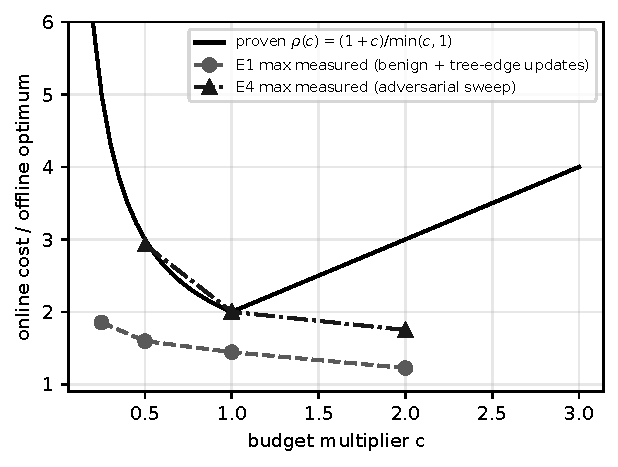
\includegraphics[width=0.95\columnwidth]{../docs/figures/fig_a_ratio_vs_rho.pdf}
\caption{Measured ratio versus the proven $\rho(c)$.}
\label{fig:a}
\end{figure}
\begin{figure}[t]
\centering
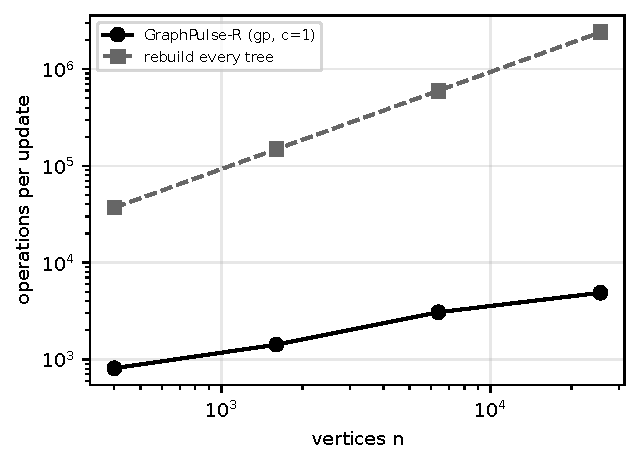
\includegraphics[width=0.95\columnwidth]{../docs/figures/fig_c_scaling.pdf}
\caption{Operations per update versus graph size (log--log).}
\label{fig:c}
\end{figure}

\section{Discussion and Limitations}
\begin{enumerate}
\item The proven work bound and competitive ratio hold for an \emph{oracle} estimate of $F$, which costs a full rebuild to obtain; the deployable mode reuses the last observed $F$ and has no theorem.
\item The offline optimum is taken per update as $\min(r,F)$; this reduction relies on the maintained state being canonical, which we checked empirically but have not proved.
\item Updates are increase-only; insertions and weight decreases are out of scope.
\item The exact tour layer is limited to $k\le 18$ stops (Held--Karp memory); the problem is NP-complete in general.
\item The implementation is pure Python and graphs are small; we make no scalability claim.
\item Only synthetic graphs were used; no real road network was evaluated.
\item On workloads where most updates touch the incumbent tour, the lazy certificate saves little; the tables report such cases rather than hiding them.
\item The adversarial family does not demonstrate the bound for the largest budget.
\end{enumerate}

\section{Conclusion}
We integrated a structural certificate, budgeted repair with a free abort, and a lazy tour certificate into one exact pipeline, proved a work bound and a competitive ratio for the shortest-path layer, and evaluated the system end to end in operation counts. The evaluation is limited to synthetic graphs and small $k$, and the literature check is still open.

\bibliographystyle{IEEEtran}
\bibliography{refs}

\end{document}
